% TODO design "brief" function to compile a more compact version of this CV
% TODO define manual Vim folds; but I think the latex plugin overrides the fold expression

% Load my custom CV class
\documentclass{cv}

% Initialize variables
\setthemecolor{Red}
\addbibresource{cv.bib}

% Define string versions of your author name to automatically make it bold in the bibliography
\setboldnames{{Edwin Wenink}, {E.~Wenink}, {Wenink, E}, {Wenink, Edwin}}


%%% Begin Document
%%% ------------------------------------------------------------
\begin{document}

% you can upload a photo and include it here...
\begin{wrapfigure}{r}{0.2\textwidth}
	\vspace*{-5em}
	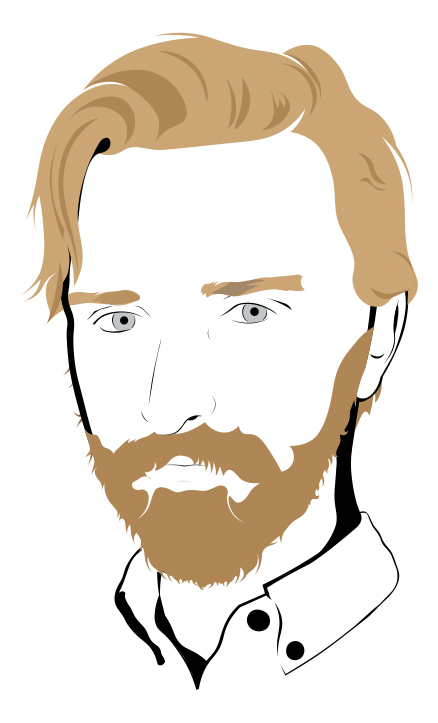
\includegraphics[width=0.15\textwidth]{img/ejw.jpg}
\end{wrapfigure}

% Set stretch
\baselinestretch

\MyName{Edwin Wenink}
\MySlogan{Curriculum Vitae}

\sepspace

%%% Personal details
%%% ------------------------------------------------------------
\NewPart{Personal details}{}

\PersonalEntry{Name}{E.J. Wenink}
\PersonalEntry{Birth}{October 3, 1993}
\PersonalEntry{Mail}{\url{edwinwenink@hotmail.com}}
\PersonalEntry{Github}{\url{https://github.com/EdwinWenink}}
\PersonalEntry{LinkedIn}{\url{https://www.linkedin.com/in/ejwenink/}}
\PersonalEntry{Website}{\url{https://www.edwinwenink.xyz}}
%\PersonalEntry{Telephone}{06-XXXXXXXX}


%%% Education
%%% ------------------------------------------------------------
\NewPart{Education}{}

\EducationEntry{Master Artificial Intelligence}{2019-2022}{Radboud University}{Specialisation: Intelligent Technology\\
Thesis title: \emph{On the explainability of case law recommendations using paragraph embeddings}\\
Supervisors: Prof. dr. Tom van Engers and dr. Johan Kwisthout\\
GPA: 8.7\footnote{On a scale from 1 to 10.}, \emph{Cum laude}}


\EducationEntry{Research Master Philosophy}{2014-2020}{Radboud University}{Specialisation: Metaphysics and Epistemology\\
Thesis title: \emph{Destiny and adestination: Derrida and Heidegger on the sending of being}\\
Supervisor: Prof. dr. Gert-Jan van der Heiden\\
GPA: 8.3, \emph{Bene meritum}}


\EducationEntry{Bachelor Artificial Intelligence}{2016-2019}{Radboud University}{Thesis title: \textit{Query by Navigation over Legal Documents:\\
An Automated Pipeline using Formal Concept Analysis} \\
Supervisor: dr. Franc Grootjen, in cooperation with Wolters Kluwer \\
GPA: 8.7, \emph{Cum laude}}


\EducationEntry{Honours Programme Philosophy, Theology\\ and Religious Studies}{2012-2014}{Radboud University}{On Schopenhauer's pessimistic metaphysics\\ Supervisor: Prof. dr. Ger Groot}


% NOTE do not split up entry over two pages
% TODO way to do this automatically?
\newpage
\EducationEntry{Bachelor Philosophy}{2011-2014}{Radboud University}{Thesis title: \textit{Van Stem naar Arche-Schrift: Deconstructie in} De la Grammatologie\\
Supervisor: Prof. dr. Philippe van Haute\\
GPA: 8.8, \emph{Cum laude}}


\EducationEntry{Gymnasium}{2005-2011}{Thomas a Kempis college, Arnhem}{Graduated in two curricula: Nature and Technology, Nature and Health.\\ GPA: 8.5
}

%%% Honours, prizes, scholarships, grants
%%% ------------------------------------------------------------
%\NewPart{Honours}{}

%\sepspace

%%% Work experience
%%% ------------------------------------------------------------
\NewPart{EXPERIENCE}{}

%%% ------------------------------------------------------------
\subsection*{1. Internships}

\WorkEntry{Graduate Research Intern Explainable AI}{Sep.2021-Apr.2022}{TNO: Netherlands Organisation for Applied Scientific Research}{I worked on explainable recommendation of case law using text mining, embeddings, and counterfactual explanations. The internship took place within FATE, a flagship project of TNO's \href{https://appl-ai-tno.nl/}{\emph{Appl.ai}} program. FATE stands for FAir, Transparent and Explainable decision making.}

\WorkEntry{Intern Innovation Platform}{Mar.2021-Aug.2021}{NS: Netherlands Railways}{I helped realize an ethical approach to AI at NS by 1) working on AI policy and making it applicable to developers (ethics by design) and 2) researching tools and techniques for implementing values such as explainability and fairness.}


%%% ------------------------------------------------------------
\subsection{Teaching and Tutoring}

\WorkEntry{Teaching Assistant Ethics for AI}{Mar.2021-Jul.2021}{Radboud University Nijmegen}{Chair working groups in the AI master\\ and contribute exam questions}


\WorkEntry{Teaching Assistant Societal Impact of AI}{Sep.2019-Feb.2020}{Radboud University Nijmegen}{Responsibilities: Teach working groups\\ and grade assignments and exams }


\WorkEntry{Teaching Assistant Introduction Artificial Intelligence}{Sep.2019-Nov.2019}{Radboud University Nijmegen}{Responsibilities: Teach working groups }


\WorkEntry{Teaching Assistant Theoretical Cognitive Science}{Feb.2019-Sep.2019}{Radboud University Nijmegen}{Responsibilities: Teach working groups\\ and grade assignments and exams }


\WorkEntry{Freelance Tutor for Student Recruitment Philosophy}{2014-2017}{Radboud University Nijmegen}{Chair working groups on university taster days}


\WorkEntry{Tutor in logic for philosophy students}{2011-2013}{}


\WorkEntry{Tutor in mathematics for high school students}{2009-2013}{}


%%% ------------------------------------------------------------
\subsection{Academic appointments}

\WorkEntry{Student Evaluation for the NVAO\\ Accreditation of Artificial Intelligence}{Nov.2018-Jan.2019}{Radboud University Nijmegen}{I was invited to participate in the self-evaluation\\of the study programme Artificial Intelligence\\ as needed for the accreditation by NVAO (every six years)}


\WorkEntry{Member of the Education Committee\\ Research Master Philosophy}{2015-2016}{Radboud University Nijmegen}{Main tasks: Reviewing the curriculum and providing recommendations\\ in cooperation with other advisory organs and the faculty board,\\ organizing social activities}


\WorkEntry{Member Nomination Committee for Assistant\\ Professor of the History of Philosophy}{Mar.2016}{Radboud University Nijmegen}{I was the student member of the nomination committee\\ that reviewed the candidate for the position of\\ Assistant Professor of the History of Philosophy}


\WorkEntry{Chairman on the Annual Deleuze Scholarship Conference}{Jun.2015}{Edition 4: Deleuze \& Aesthetics}{I chaired the parallel session ``Decentering subject matter'' }


%%% Skills
%%% ------------------------------------------------------------
\NewPart{Skills}{}

\SkillsEntry{Programming Languages}{\textbf{\emph{Experienced:}} Python \halfpipe \textbf{\emph{Familiar:}} Java \halfpipe R \halfpipe Bash \halfpipe SQL \halfpipe \LaTeX}

% Hugo? HTML5? CSS? TODO avoid overflowing into left column!
\SkillsEntry{Frameworks \& Libraries}{Scikit-learn \halfpipe NumPy \halfpipe Pandas \halfpipe NLTK \halfpipe Gensim \halfpipe PyTorch \halfpipe TensorFlow}

\SkillsEntry{Software dev.}{Programming paradigms \halfpipe Git \halfpipe CLI \halfpipe Agile \halfpipe Unix \halfpipe Vim}

\SkillsEntry{Languages}{\textbf{\emph{Native:}} Dutch \halfpipe \textbf{\emph{Fluent:}} English \halfpipe \textbf{\emph{Conversational:}} German}

% TODO soft skills; project management; 


%%% ------------------------------------------------------------
\NewPart{Papers and talks}

\subsection{Papers}

\nocite{*}
\printbibliography[heading=none]

% TODO automatically make "Edwin Wenink" bold
% See for BibTex (but I use biblatex):  https://yuzhangbit.github.io/tools/highlighting-author-name-for-IEEEtran-style/
% biblatex.cfg customization: https://tex.stackexchange.com/questions/12806/guidelines-for-customizing-biblatex-styles
% define "Edwin Wenink" as a variable somewhere to make the .cls file more general
% Solution for BibLatex: https://answerbun.com/ -> "Make specific author bold using biblatex"

% TODO could also refer to my main bib file; then filter out refs with "Edwin Wenink" as an author

% TODO to later distinguish journal from conference papers, use something like this to automatically separate them from a single bib file
% \subsection*{Journal articles}
% \begin{refcontext}[labelprefix=J]
% \printbibliography[type=article]
% \end{refcontext}

% \subsection*{Conference publications}
% \begin{refcontext}[labelprefix=C]
% \printbibliography[type=inproceedings]

\subsection{Talks}

\WorkEntry{``E-Salon: social media, zegen of vloek voor het vrije debat?''}{2021}{Invited speaker by Stichting Vrij Links.\\
Event page: \url{https://www.vrij-links.nl/e-salon/social-media-zegen-of-vloek-voor-het-vrije-debat/}}

\WorkEntry{``Kunstmatige Intelligentie en haar gevolgen''}{2020}{Invited guest on the podcast \href{https://vocast.live/aflevering/kunstmatige-intelligentie/}{Vocast}}

\WorkEntry{``Metaphysics and Metaphor in Heidegger's works''}{2016}{Joint Symposium of F.C. Sophia and Student Recruitment}

\WorkEntry{Lecture (90 min.) on Schopenhauer's metaphysics\\
in \textit{Die Welt als Wille und Vorstellung}}{2012}{Graduation component of my honours programme}

%%% project
%%% ------------------------------------------------------------
\NewPart{Projects}{}

\WorkEntry{Archive Fever: Website on Philosophy, Technology and AI}{2018-Present}{Editor, developer and writer}{Published 70+ online articles ranging from\\
	technical tutorials to philosophical essays.\\
	Currently 72.336 page views and 848 monthly unique visitors\\
	Hosted at \url{https://www.edwinwenink.xyz}
}

\WorkEntry{The AI Ethics Tool Landscape}{2021}{Editor, developer}{An open-source project that builds a taxonomy of practical tools for\\
implementing ethical AI.\\
Hosted at \url{https://edwinwenink.github.io/ai-ethics-tool-landscape/}}

\WorkEntry{Elecast: Navigating Podcasts}{2020}{Developer}{A podcast app that allows navigation from audio segments to the\\ corresponding location in an AI-generated transcript and \textit{vice versa}.\\
Progressive Web App implemented in React.\\
Prototype at \url{https://nml-podcast-transcription.now.sh/player}}


\WorkEntry{CLIDE: A Clean IDE within Eclipse}{Sep.18-Feb.19}{Product owner by proxy, developer}{Scrum development of an IDE for the Clean functional\\ 
programming language, as an extension to the Eclipse framework.\\
As a product owner by proxy, I established product requirements\\
and priorities together with the client. \\
For information on Clean, see \url{https://clean.cs.ru.nl/Clean}}


\vspace*{\fill}

\noindent\small Last updated on \today.\\
\\
\noindent\small Complete list of followed university courses available @ \url{https://www.edwinwenink.xyz/etc/courses/}\\
\noindent\small (La)TeX source files @ \url{https://github.com/EdwinWenink/cv} \\

\end{document}
